%%
%% kit-prog-tutorial
%%
%% Slides for my Java programming tutorial at KIT using LaTeX beamer.
%%
%% Copyright (c) 2015-2016 YouniS Bensalah <younis.bensalah@gmail.com>
%%
%% This work is released to the public domain.
%% For the full copyright and license information, please view the LICENSE file.
%%

\documentclass[18pt]{beamer}

\usepackage{templates/beamerthemekit}

\usepackage[utf8]{inputenc}
\usepackage{hyperref}
\usepackage{listings}
\usepackage{xcolor}
\usepackage{colortbl}

\titleimage{road}

\definecolor{lime}{HTML}{8FFF53}

\newcommand{\tagline}{Exceptions}

\newcommand{\quotes}[1]{``#1''}

\title[Programmieren\hspace{2.5pt}--\hspace{2.5pt}\tagline]{\tagline}
\subtitle{Programmieren~\textbar~Tutorium 32}

\author{YouniS Bensalah}
\date{16. Januar 2017}

\institute{Chair for Software Design and Quality}

\usepackage[citestyle=authoryear,bibstyle=numeric,hyperref,backend=biber]{biblatex}
\addbibresource{templates/example.bib}
\bibhang1em

\begin{document}

% remove annoying figure prefix in caption
\setbeamertemplate{caption}{\raggedright\insertcaption\par}

\selectlanguage{english}

\begin{frame}
    \titlepage
\end{frame}

% \begin{frame}{Heute}
%     \tableofcontents
% \end{frame}

\section{Exceptions}

\begin{frame}{Exceptions}
    \begin{block}{}
        \begin{itemize}
            \item \textit{Exceptions} dienen der Ankündigung und Behandlung von \textbf{Ausnahmesituationen}
            (e.g., Fehler, unerwartete Ergebnisse) innerhalb eines Programms
            \item Dabei kann die Information über die Ausnahmesituation an eine andere Programmebene zur Behandlung übergeben werden
        \end{itemize}
    \end{block}

\end{frame}

\begin{frame}{Exceptions}
    \textit{Was passiert jetzt also bei einem Fehler?}
    \vspace{.2in}
    \begin{enumerate}
        \item Das Programm meldet den Vorfall in dem es eine \textbf{Exception} \textit{wirft}
        \item Der \quotes{normale} Kontrollfluss wird unterbrochen und es wird nach einem Zuständigen gesucht, der den Fehler behandelt
        \item Wenn dieser existiert, dann wird die Exception \textit{aufgefangen} und der entsprechende Code wird ausgeführt
        (z. B. der Fehler wird geloggt, das Programm wird terminiert\dots)
    \end{enumerate}
\end{frame}


\subsection{try und catch}


\begin{frame}[fragile]{try-catch}
    \begin{itemize}
        \item In den \textbf{try}-Block kommt der Code, der potentiell eine Exception wirft
        \item Im \textbf{catch}-Block steht dann der Code, der die Exception behandelt, falls eine auftritt
        \item Nach dem \textbf{try-catch}-Block steht der Code, welcher anschließend \\
        \textit{in jedem Fall} ausgeführt wird
    \end{itemize}

    \begin{exampleblock}{Syntax}
        \begin{lstlisting}[language=Java,basicstyle=\scriptsize]
try {
    ... // code that might throw an exception
} catch (ExceptionType e) {
    ... // code that handles the exception
}
... // code that will be executed after try-catch block
        \end{lstlisting}

    \end{exampleblock}
\end{frame}

\subsection{Exception werfen mit throw}


\begin{frame}[fragile]{throw}
    \textit{Wann wird eine Exception geworfen?}
    \begin{itemize}
        \item Java wirft einige Exceptions automatisch, wenn etwas zur Laufzeit schiefläuft\dots
        \begin{itemize}
            \item \texttt{Integer.parseInt()} wirft eine \texttt{NumberFormatException}, falls das Argument keine gültige Zahl darstellt
        \end{itemize}
        \item Man kann auch selbst Exceptions werfen ! (mit \texttt{throw})
    \end{itemize}

    \begin{exampleblock}{Syntax}
throw new SomeException();
    \end{exampleblock}

    \begin{itemize}
        \item Es wird also ein \textbf{Objekt} vom Typ \texttt{SomeException} erstellt und geworfen!
    \end{itemize}

\end{frame}


\begin{frame}[fragile]{Exceptions}
    Was wird hier ausgegeben?
    \begin{exampleblock}{}
        \begin{lstlisting}[language=Java,basicstyle=\scriptsize]
public static void main(String[] args) {
    try {
        doSomething();
    } catch (ArrayIndexOutOfBoundsException e) {
        System.out.println("Oh noes!");
    }
    System.out.println("Whatever.");
}

public static void doSomething() {
    int[] foo = new int[4];
    foo[4] = 1337;
    System.out.println("I know arrays.");
}
        \end{lstlisting}

    \end{exampleblock}

\end{frame}

\begin{frame}[fragile]{Exceptions}
    \begin{exampleblock}{}
        \begin{lstlisting}
Oh noes!
Whatever.
        \end{lstlisting}

    \end{exampleblock}

    \pause

    \begin{itemize}
        \item Die Zeile \begin{lstlisting}[language=Java,basicstyle=\scriptsize]
foo[4] = 1337;
        \end{lstlisting}
        löst eine \texttt{ArrayIndexOutOfBoundsException} aus
        \item Der Kontrollfluss springt in den \texttt{catch}-Block, der diese Ausnahme abfängt
        \item Anschließend geht es \textbf{\alert{nach dem \texttt{catch}}} weiter!
        \item Die Ausgabe \quotes{\texttt{I know arrays.}} wird nie erreicht

    \end{itemize}

\end{frame}


\begin{frame}[fragile]{Exceptions}
    Was wird hier ausgegeben?
    \begin{exampleblock}{}
        \begin{lstlisting}[language=Java,basicstyle=\scriptsize]
public static void main(String[] args) {
    try {
        doMagic(42);
        System.out.println("Okay, I fixed it!");
    } catch (MagicException e) {
        System.out.println("Wrong magic.");
    }
    System.out.println("Whatever.");
}

public static void doMagic(int magic) {
    if (magic != 1337) {
        throw new MagicException();
    }
    System.out.println("Do magic...");
}
        \end{lstlisting}

    \end{exampleblock}

\end{frame}

\begin{frame}[fragile]{Exceptions}
    \begin{exampleblock}{}
        \begin{lstlisting}[language=Java]
Wrong magic.
Whatever.
        \end{lstlisting}

    \end{exampleblock}

\end{frame}

\begin{frame}{Exceptions}
    \alert{\huge{\textsc{Nach einer aufgefangenen Exception geht es immer nach catch weiter!!!}}}
\end{frame}

\subsection{Checked versus Unchecked}


\begin{frame}{Eigene Exceptions}
    \begin{itemize}
        \item Man kann die \quotes{built-in} Exceptions von Java verwenden:
        \begin{itemize}
            \item \texttt{IllegalArgumentException}
            \item \texttt{UnsupportedOperationException}
            \item \texttt{IndexOutOfBoundsException}
            \item \texttt{IllegalStateException}
            \item \dots
        \end{itemize}
        \vspace{.2in}
        \item Benötigt man eigene Exceptions, kann man die Klasse \texttt{Exception} bzw. \texttt{RuntimeException} \textbf{erweitern}.
    \end{itemize}

\end{frame}


\begin{frame}{Checked vs. Unchecked Exceptions}
    In Java gibt es \textbf{checked} und \textbf{unchecked} Exceptions.
    \vspace{.2in}
    \begin{itemize}
        \item \textbf{Checked Exceptions}
        \begin{itemize}
            \item Ausnahmesituation oder Problem, dessen Ursache \textbf{außerhalb} des Zuständigkeitsbereichs des aktuellen Moduls liegt
            \item \textit{Ungültige Benutzereingabe, Datenbank-Problem, nicht vorhandene Datei \dots}
            \item Müssen \textbf{immer} abgefangen werden und durch \texttt{throws} kenntlich gemacht werden
            \item Unterklassen von \texttt{Exception}
        \end{itemize}
    \end{itemize}

\end{frame}

\begin{frame}{Checked vs. Unchecked Exceptions}

    \begin{itemize}
        \item \textbf{Unchecked Exceptions}
        \begin{itemize}
            \item Ausnahmesituation oder ungültiger Zustand, dessen Ursache meistens ein Bug im Programmcode selbst ist
            \item In den meisten Fällen kann das Programm dann ohnehin nicht sinnvoll weiterlaufen
            \item \textit{Ungültige Argumente, division by 0, ungültiger Index bei Zugriff auf Array \dots}
            \item Können, müssen aber nicht abgefangen werden
            \item Unterklassen von \texttt{RuntimeException}
        \end{itemize}
    \end{itemize}

\end{frame}


\begin{frame}{Checked vs. Unchecked Exceptions}

    \begin{itemize}
        \item \texttt{RuntimeException} ist auch Unterklasse von \texttt{Exception}
    \end{itemize}


    \vspace{.2in}

    \begin{figure}
        
\includegraphics[scale=.5]{img/whoa.jpg}
    \end{figure}

\end{frame}

\begin{frame}[fragile]{throws}

    \begin{itemize}
        \item Methoden, die \textbf{checked Exceptions} werfen können, müssen mit \texttt{throws} kenntlich gemacht werden
    \end{itemize}


    \begin{exampleblock}{Syntax}
        \begin{lstlisting}[language=Java,basicstyle=\scriptsize]
public void foo() throws SomeCheckedException {
    ...
}
        \end{lstlisting}

    \end{exampleblock}

\end{frame}

\begin{frame}{Exceptions}
    \begin{itemize}
        \item Eine \textbf{Exception} ist eine \alert{Ausnahmesituation!}
        \item \textbf{Exceptions} sollten nicht den normalen Kontrollfluss steuern
    \end{itemize}
\end{frame}

\begin{frame}{Javadoc @throws}
    Alle Exceptions sollten mittels \texttt{@throws} im Javadoc-Kommentar kurz erklärt werden:
    \begin{itemize}
        \item Was bedeutet diese Exception für das Programm
        \item Wann wird sie von der Methode \quotes{geworfen}
    \end{itemize}
\end{frame}

\appendix
\beginbackup

\begin{frame}{Fragen?}
    \begin{figure}
        
\includegraphics[scale=.6]{img/additionalquestions.jpg}
    \end{figure}
\end{frame}

\begin{frame}{Bis nächste Woche!}
    \begin{figure}
        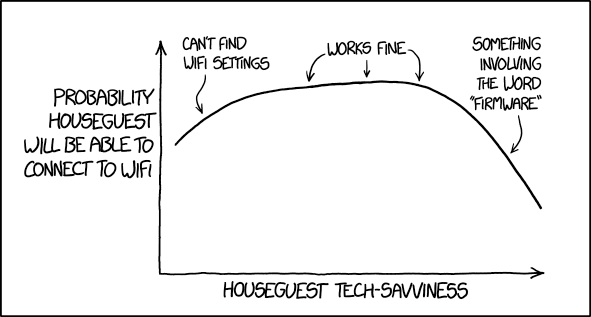
\includegraphics[scale=.5]{img/wifi.png}
        \caption{\footnotesize{xkcd.com}}
    \end{figure}
\end{frame}

\backupend

\end{document}
